\documentclass[preprint]{elsarticle}

\usepackage{lineno,hyperref}
%%\modulolinenumbers[5]
\usepackage{float}
\floatplacement{figure}{H}
\journal{Journal of Biomechanics}

%%%%%%%%%%%%%%%%%%%%%%%
%% Elsevier bibliography styles
%%%%%%%%%%%%%%%%%%%%%%%
%% To change the style, put a % in front of the second line of the current style and
%% remove the % from the second line of the style you would like to use.
%%%%%%%%%%%%%%%%%%%%%%%

%% Numbered
%\bibliographystyle{model1-num-names}

%% Numbered without titles
%\bibliographystyle{model1a-num-names}

%% Harvard
%\bibliographystyle{model2-names.bst}\biboptions{authoryear}

%% Vancouver numbered
%\usepackage{numcompress}\bibliographystyle{model3-num-names}

%% Vancouver name/year
%\usepackage{numcompress}\bibliographystyle{model4-names}\biboptions{authoryear}

%% APA style
%\bibliographystyle{model5-names}\biboptions{authoryear}

%% AMA style
%\usepackage{numcompress}\bibliographystyle{model6-num-names}

%% `Elsevier LaTeX' style
%%\bibliographystyle{elsarticle-num}
%%%%%%%%%%%%%%%%%%%%%%%

% bibliography
\bibliographystyle{elsarticle-template/model2-names.bst}\biboptions{authoryear}

\linenumbers
\usepackage{longtable}
\usepackage{booktabs}
\makeatletter
\@ifpackageloaded{subfig}{}{\usepackage{subfig}}
\@ifpackageloaded{caption}{}{\usepackage{caption}}
\captionsetup[subfloat]{margin=0.5em}
\AtBeginDocument{%
\renewcommand*\figurename{Figure}
\renewcommand*\tablename{Table}
}
\AtBeginDocument{%
\renewcommand*\listfigurename{List of Figures}
\renewcommand*\listtablename{List of Tables}
}
\@ifpackageloaded{float}{}{\usepackage{float}}
\floatstyle{ruled}
\@ifundefined{c@chapter}{\newfloat{codelisting}{h}{lop}}{\newfloat{codelisting}{h}{lop}[chapter]}
\floatname{codelisting}{Listing}
\newcommand*\listoflistings{\listof{codelisting}{List of Listings}}
\makeatother



% Scale images if necessary, so that they will not overflow the page
% margins by default, and it is still possible to overwrite the defaults
% using explicit options in \includegraphics[width, height, ...]{}
\setkeys{Gin}{width=\maxwidth,height=\maxheight,keepaspectratio}

\begin{document}



\hypertarget{figures-and-tables}{%
\section*{Figures and Tables}\label{figures-and-tables}}
\addcontentsline{toc}{section}{Figure and Tables Legends}



\hypertarget{tbl:groups}{}
\begin{longtable}[]{@{}llll@{}}
\caption{\label{tbl:groups}Enrollment groups based on reported height. 5 subjects were enrolled in each group}\tabularnewline

\end{longtable}



\begin{figure}
\hypertarget{fig:testSetup}{%
\centering
%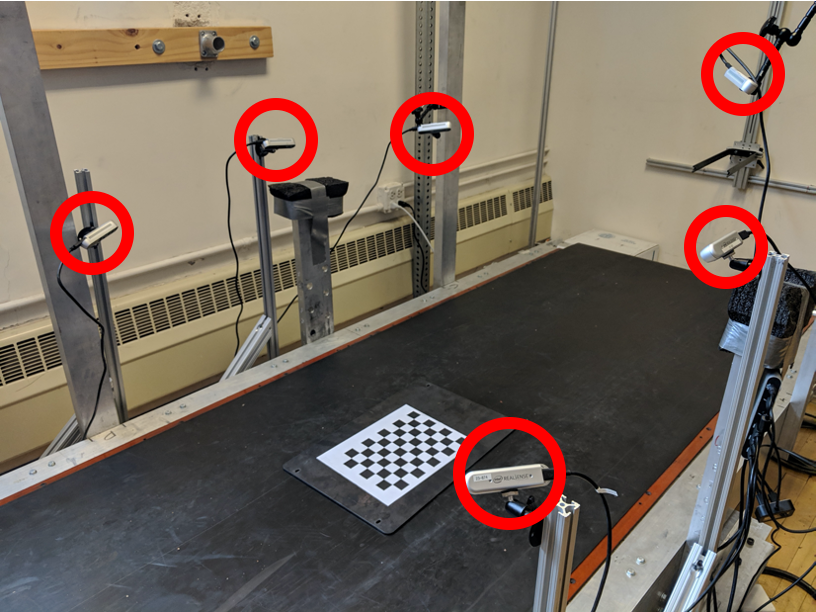
\includegraphics[width=1\textwidth,height=\textheight]{fig/capturesetup.png}
\caption{Capture setup of 6 Intel RealSense D415 Depth Cameras (circled in red) placed around a treadmill. The checkerboard shown was used to calibrate the cameras using the DynaMo package.}\label{fig:testSetup}
}
\end{figure}

\begin{figure}
\hypertarget{fig:dataflow}{%
\centering
%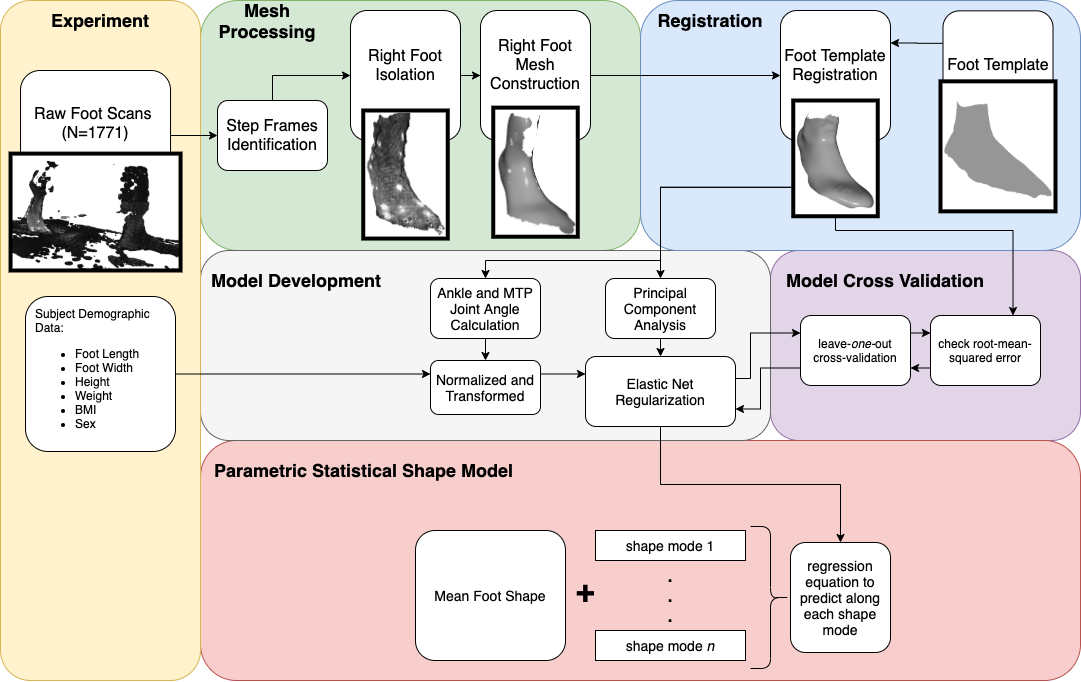
\includegraphics[width=1\textwidth,height=\textheight]{fig/footProcessing.png}
\caption{Flowchart of processing steps for statistical shape model creation}\label{fig:dataflow}
}
\end{figure}

\begin{figure}
\hypertarget{fig:scans}{%
\centering
%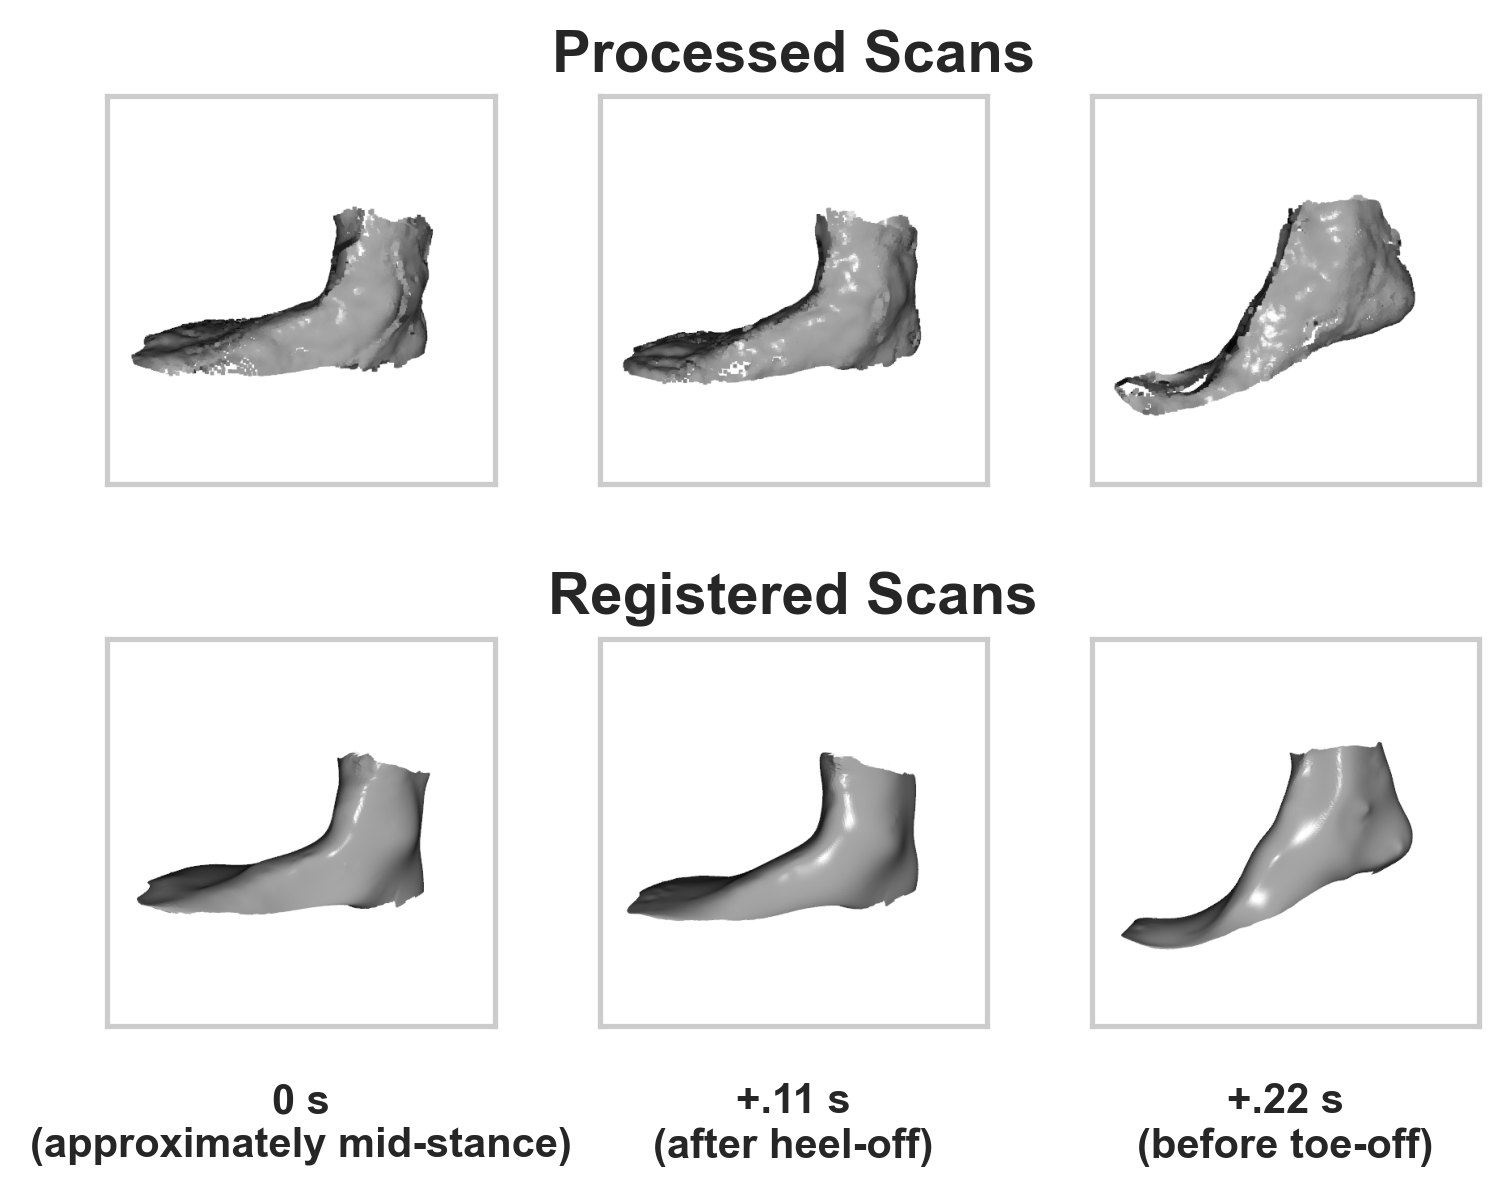
\includegraphics[width=1\textwidth,height=\textheight]{fig/scans.png}
\caption{Processed and registered scans of one subject during heel-off, shown 10 frames (.11 seconds) apart}\label{fig:scans}
}
\end{figure}

\begin{figure}
\hypertarget{fig:modelperf}{%
\centering
%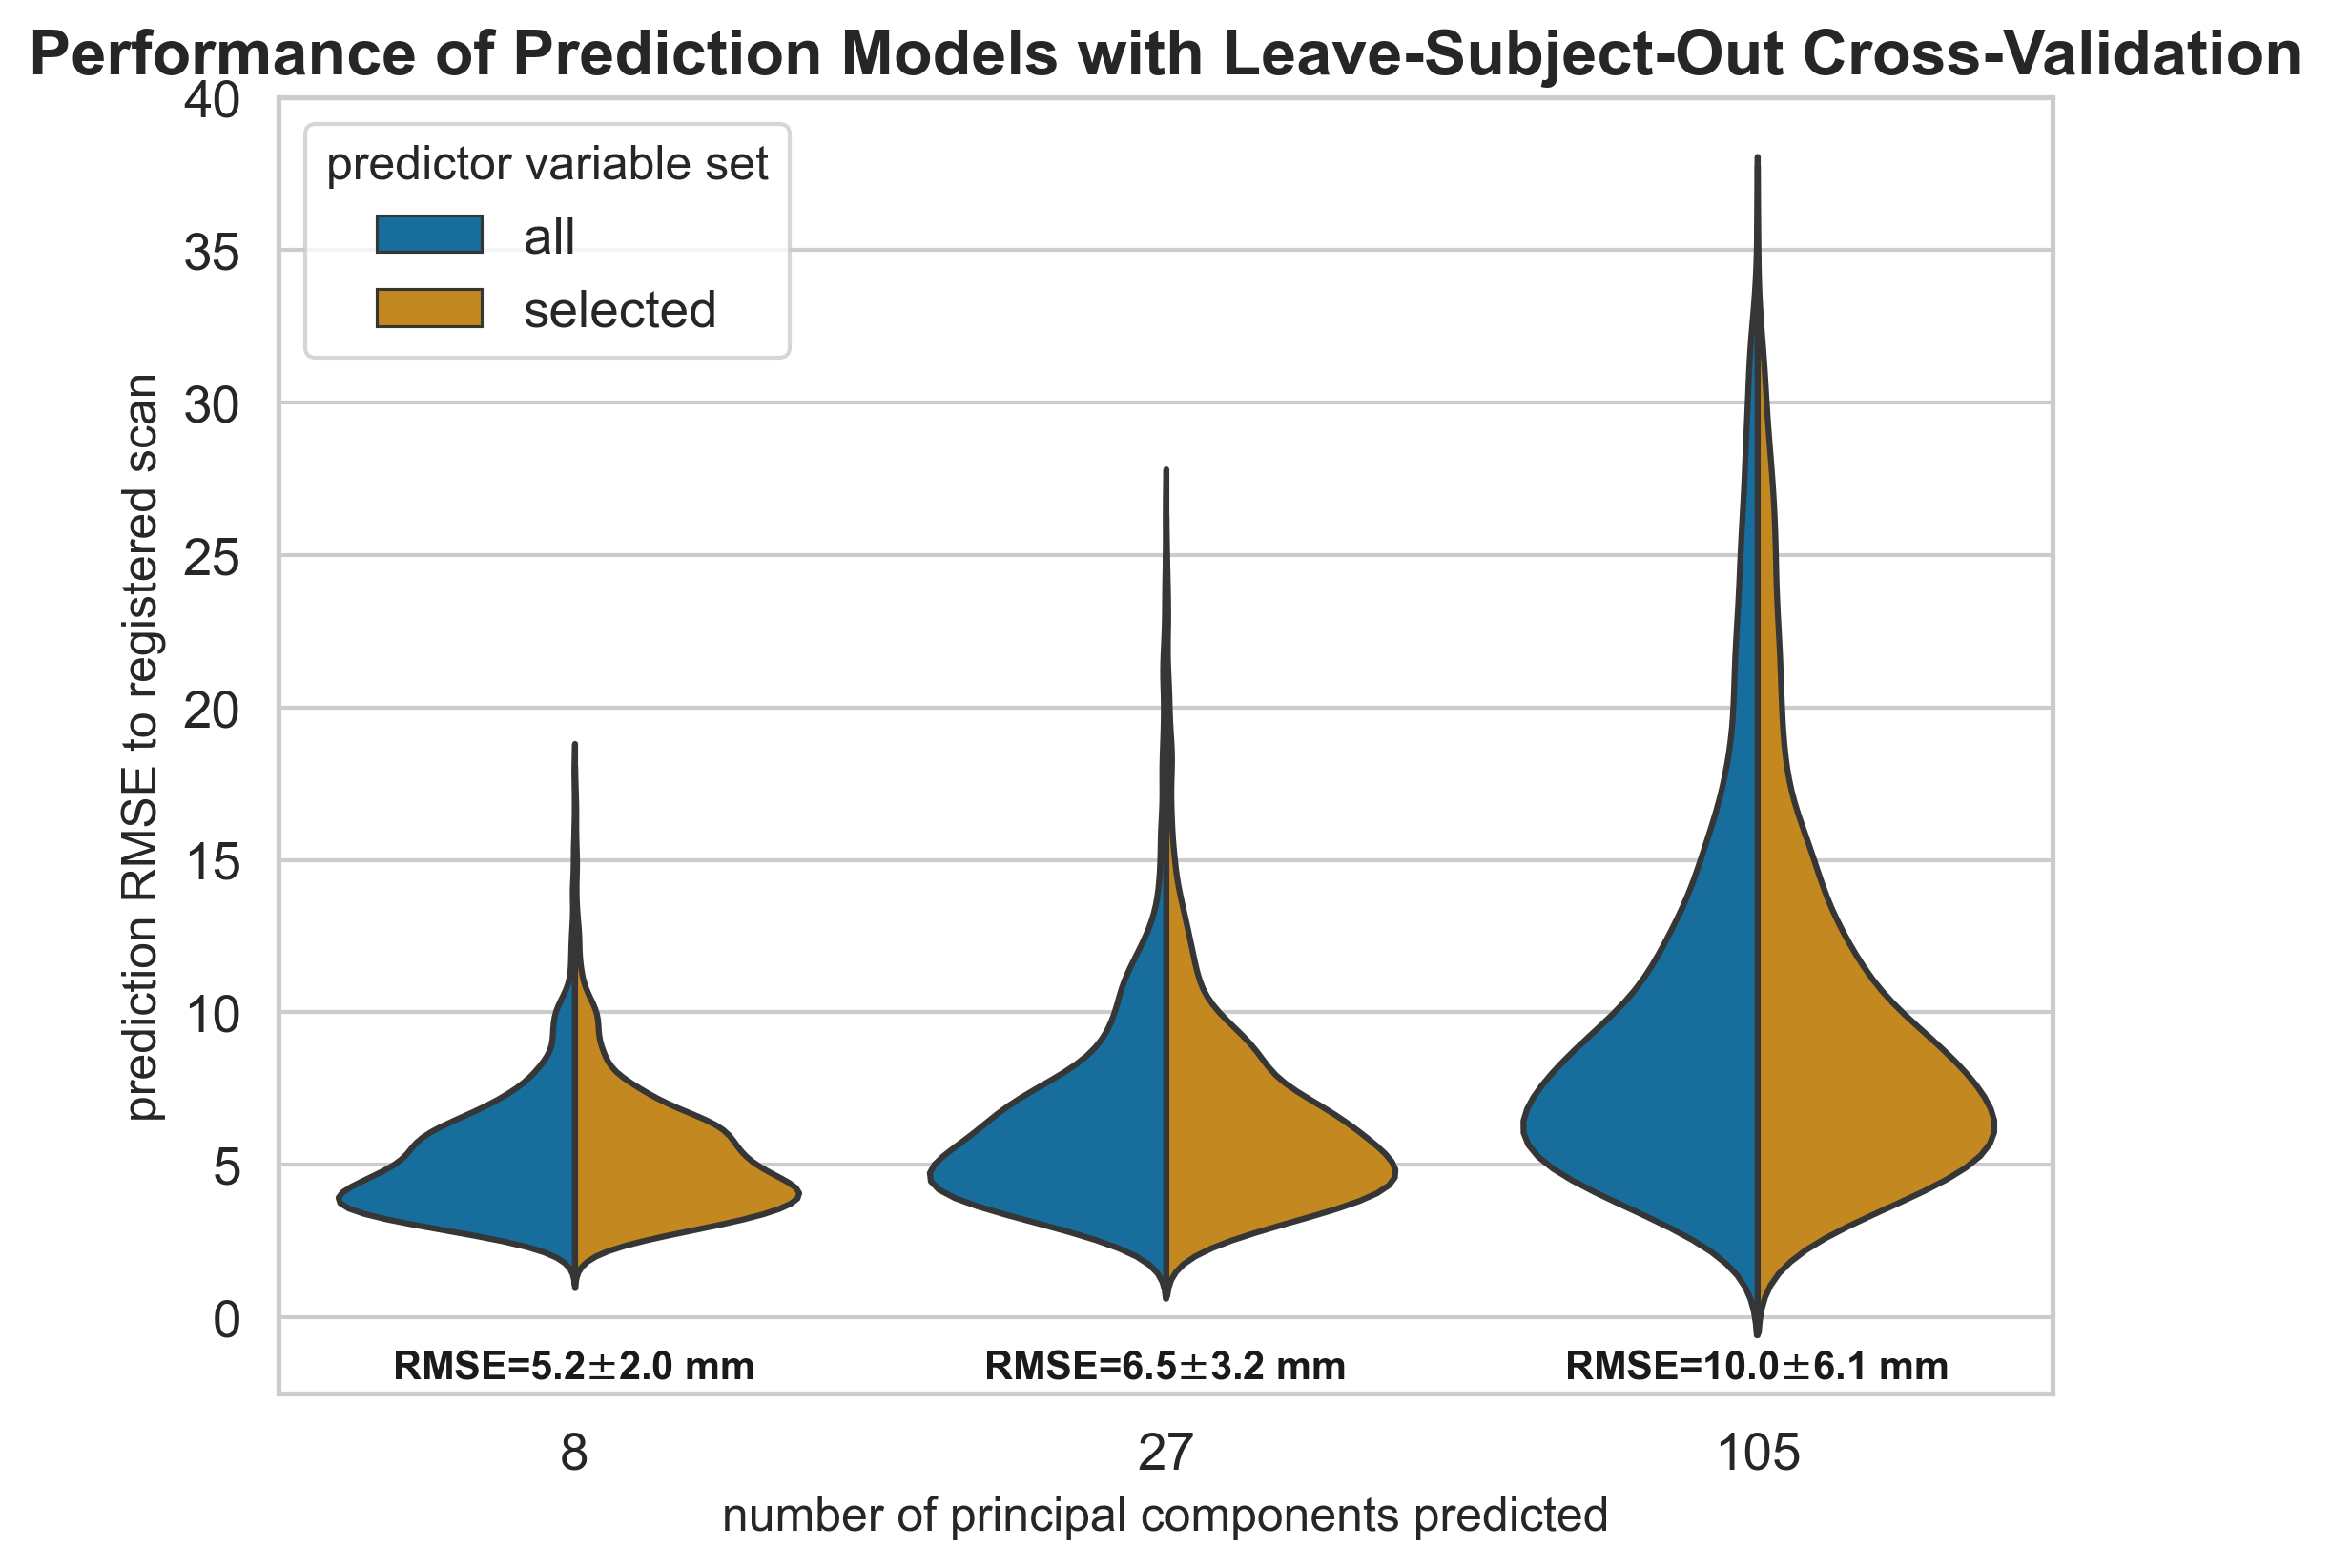
\includegraphics[width=1\textwidth,height=\textheight]{fig/modelPerformance.png}
\caption{Distribution of errors across the various prediction models leave-subject-out cross-validation results. Model RMSE mean and standard deviation are shown above each distribution}\label{fig:modelperf}
}
\end{figure}

\begin{figure}
\hypertarget{fig:coefs}{%
\centering
%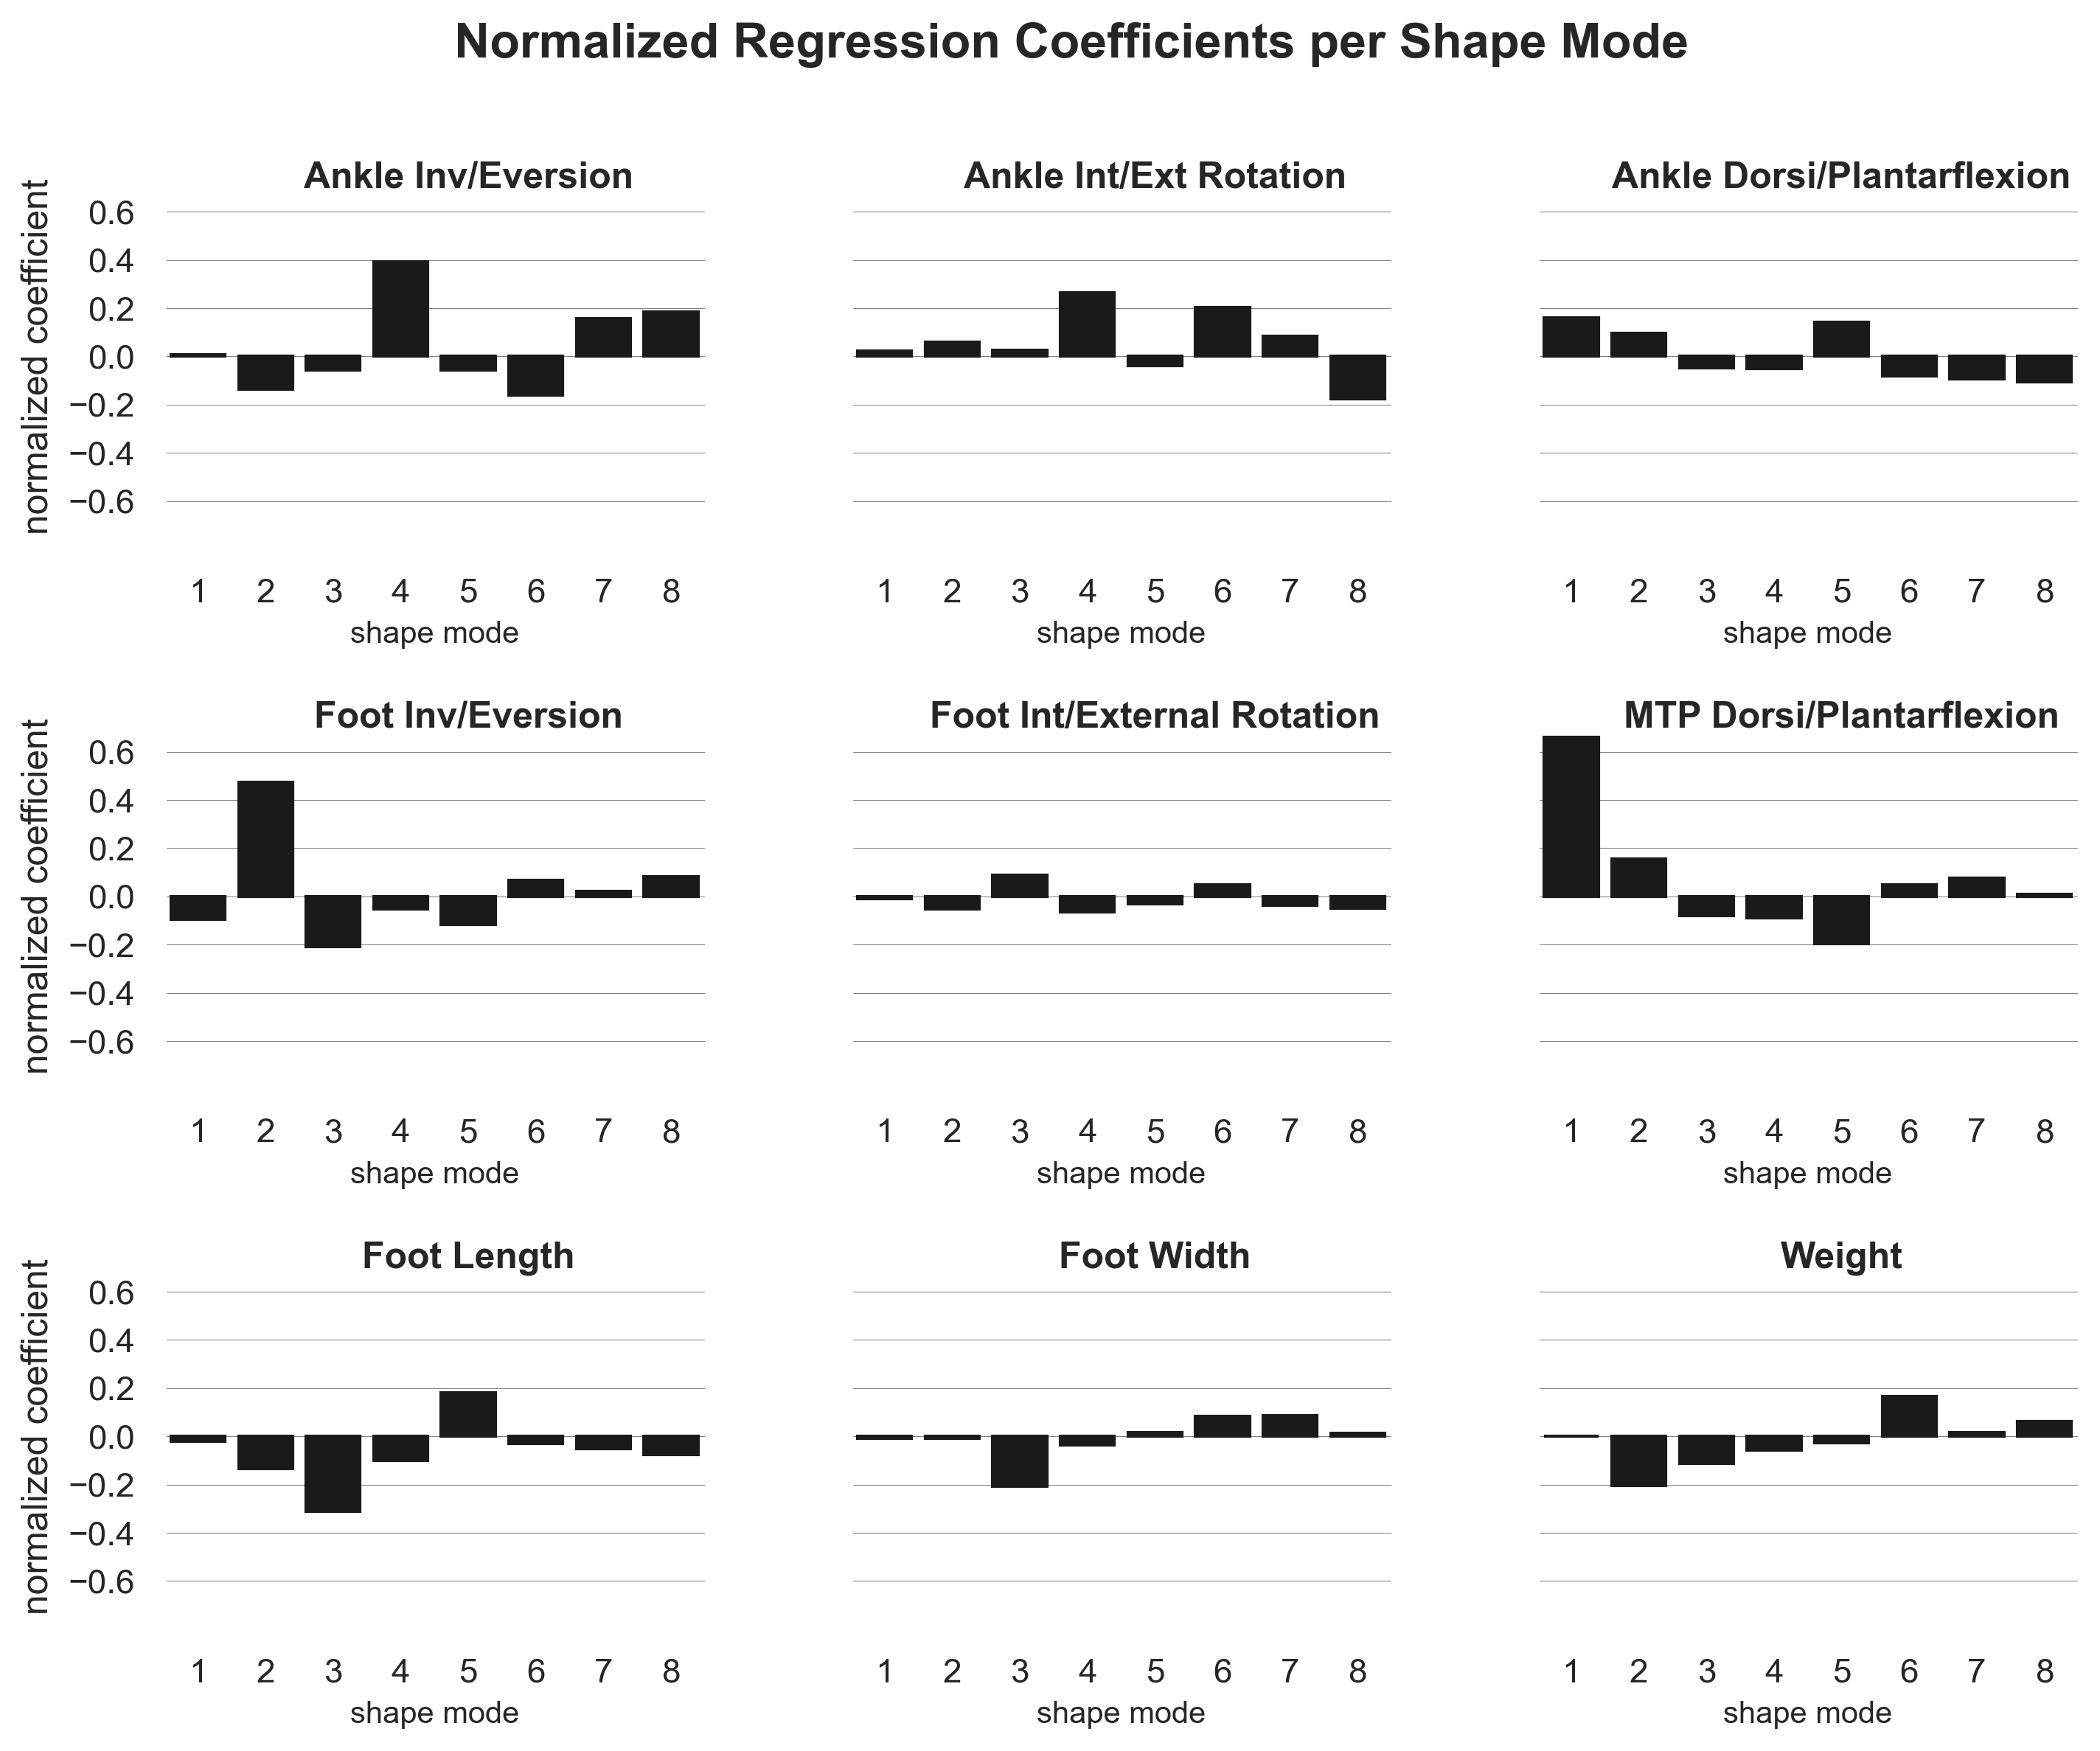
\includegraphics[width=1\textwidth,height=\textheight]{fig/coefs.png}
\caption{Each graph represents the predictor's effects on the shape mode by visualizing the model's normalized coefficients. Larger absolute values indicate a larger effect from the predictor on the shape mode.}\label{fig:coefs}
}
\end{figure}

\begin{figure}
\hypertarget{fig:pca_quad}{%
\centering
%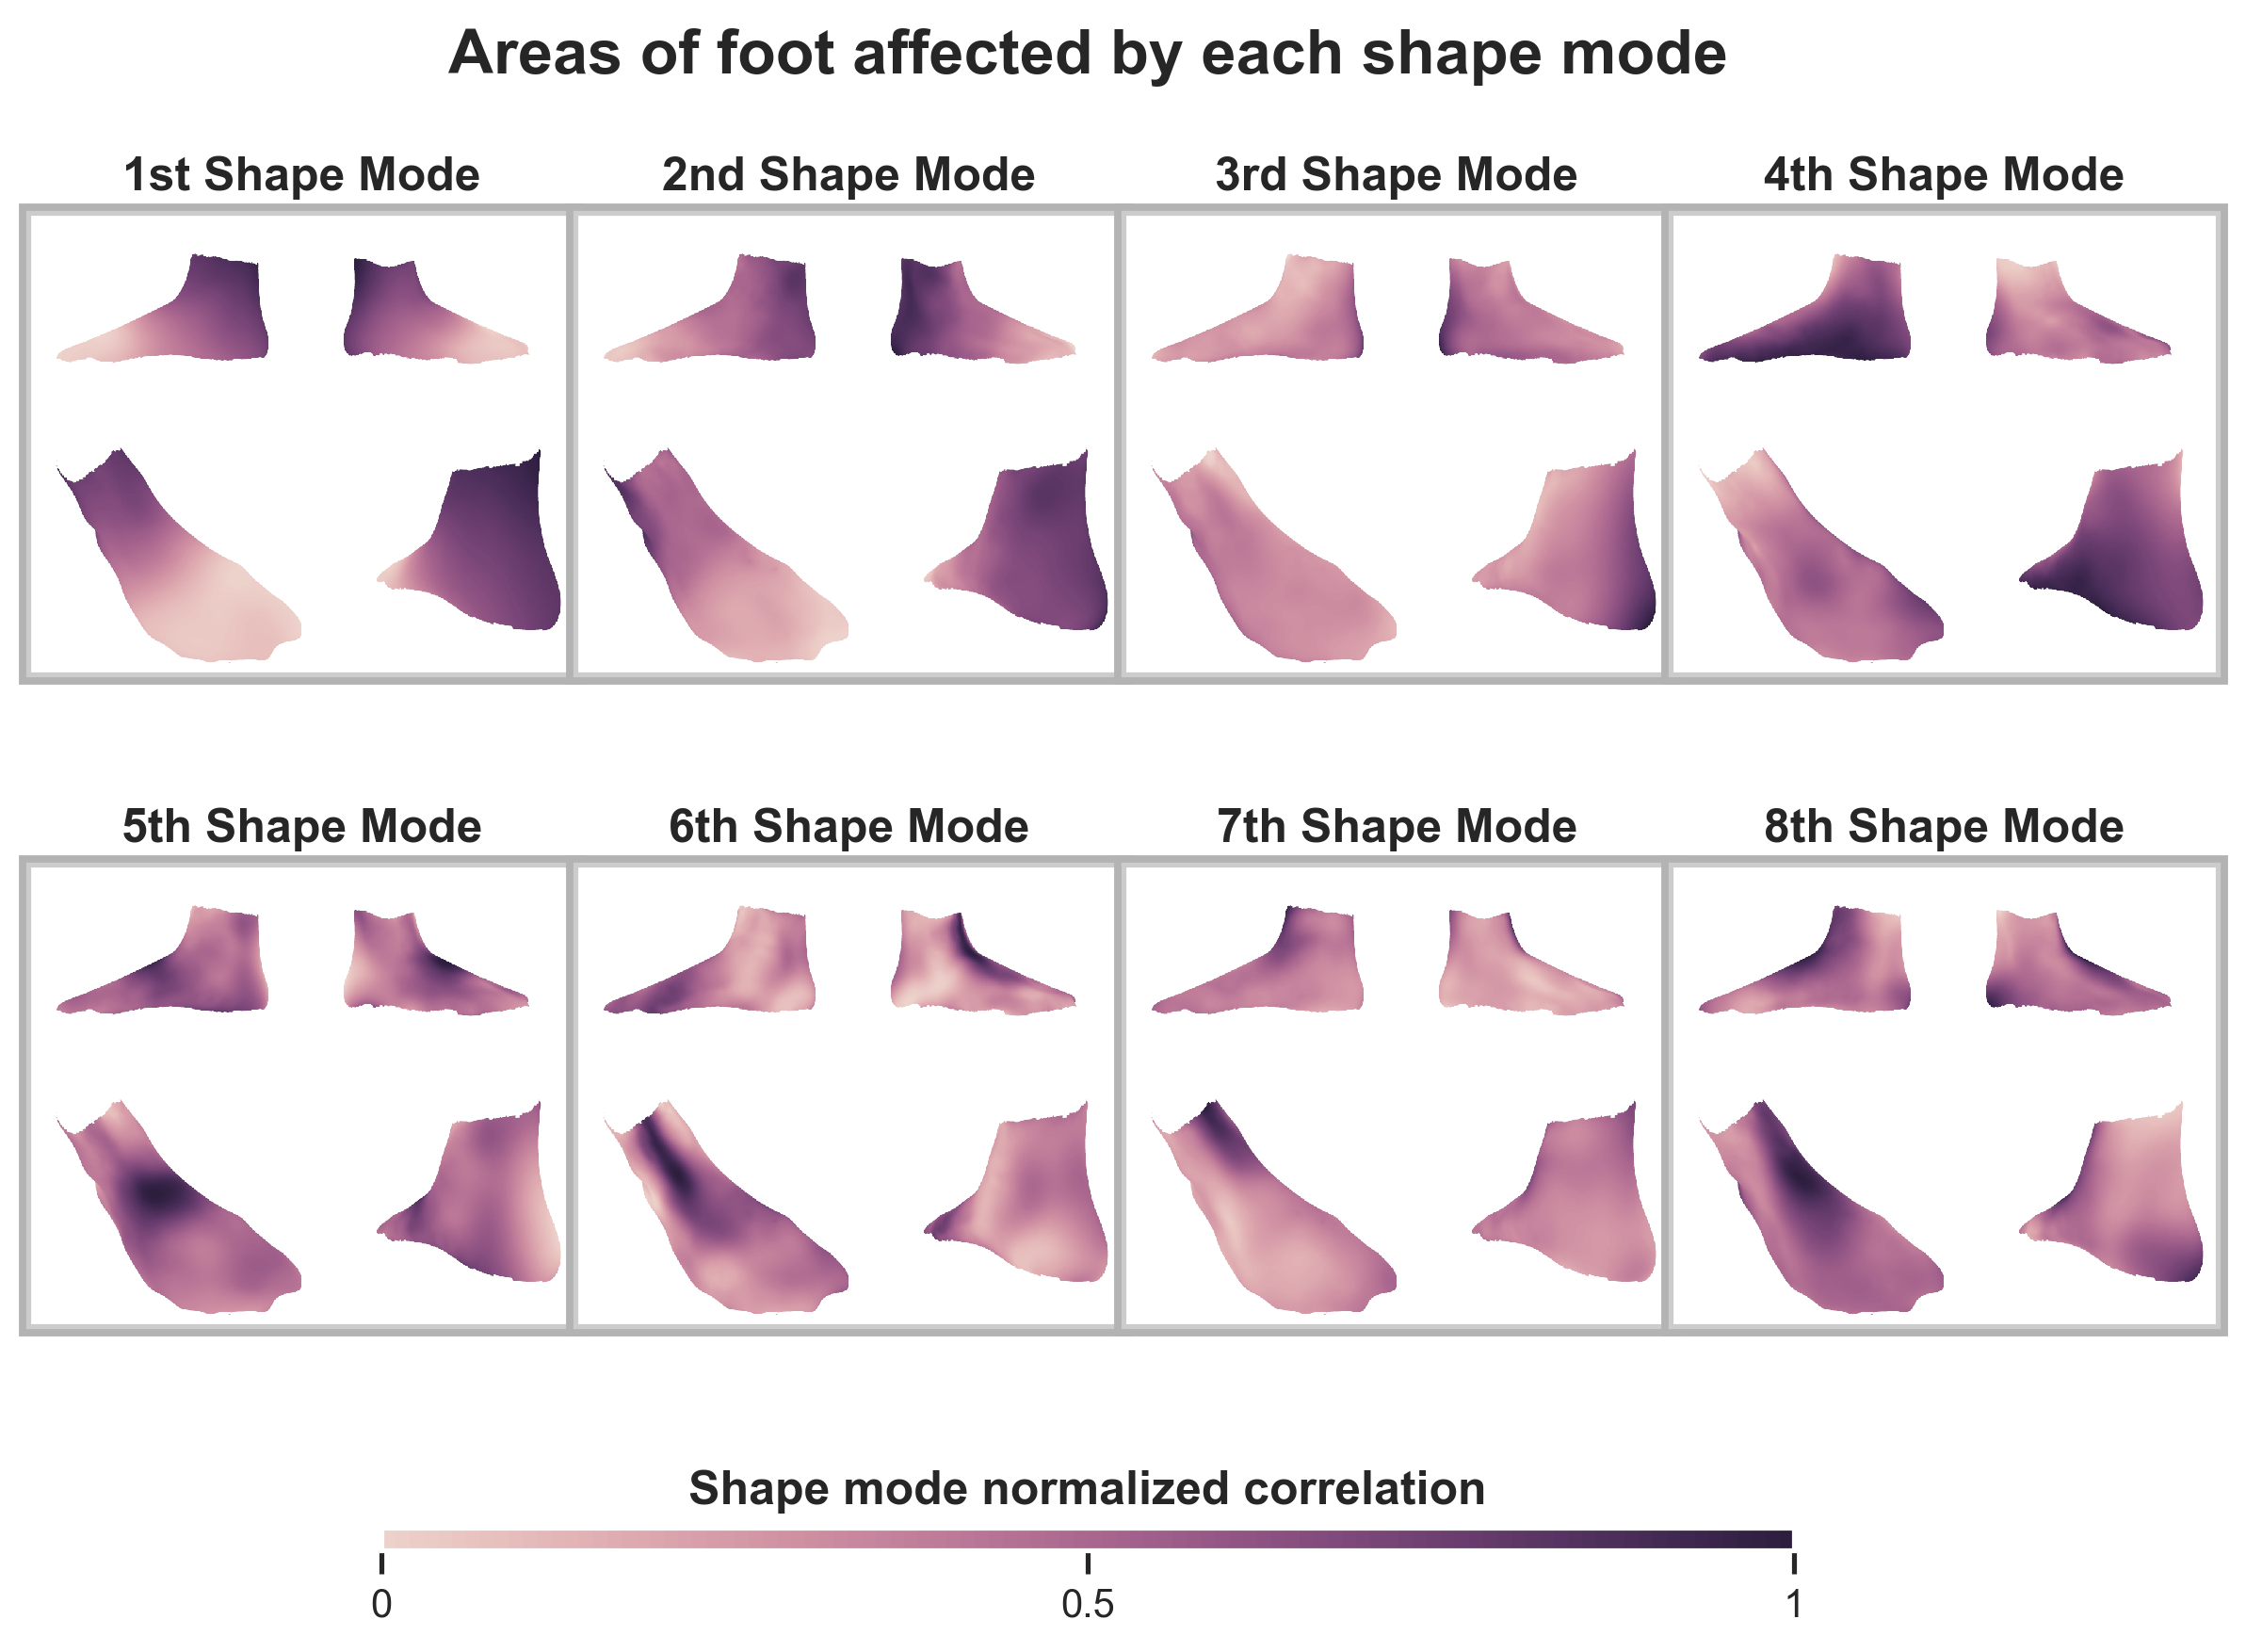
\includegraphics[width=1\textwidth,height=\textheight]{fig/PCQuad.png}
\caption{Each shape mode's principal axis represented as a heatmap overlaid on the mean foot and shown from 4 different point-of-views. The darker regions represent vertices which are most correlated with the shape mode's principal axis, and therefore see deformations in the shape mode.}\label{fig:pca_quad}
}
\end{figure}

\begin{figure}
\hypertarget{fig:pca_overlay}{%
\centering
%\includegraphics[width=1\textwidth,height=\textheight]{fig/PCVAR.png}
\caption{Foot shape deformation at +2 and -2 standard deviations along each shape mode's principal axis, overlaid on the mean foot. The point-of-view is set to highlight the major variance along each shape mode's axis.}\label{fig:pca_overlay}
}
\end{figure}


\end{document}  